\documentclass[a4paper]{article}
% Packages
\usepackage{amsmath} % For math symbols and equations
\usepackage{amssymb} % For math symbols
\usepackage{enumerate} % For custom numbering of lists
\usepackage{bm}
\usepackage{cancel} % for extra in math
\usepackage[
  inner=2cm, % Set inner margin to 2 cm
  outer=2cm, % Set outer margin to 2 cm
  bindingoffset=0.5cm, % Set binding offset to 0.5 cm
  top=2cm, % Set top margin to 2 cm
  bottom=2cm % Set bottom margin to 2 cm
]{geometry}
\usepackage{fancyhdr} % For custom headers and footers
\usepackage{lastpage} % For referencing the last page number
\usepackage{titlesec} % For custom section and subsection headings
\usepackage[version=4]{mhchem} % Required package for chemical equations
\usepackage{hyperref} % connections
\usepackage{parskip} % skip paragraphs
\usepackage[
backend=biber,
sorting=anyvt,
style = ieee
]{biblatex} % for using references
\usepackage{setspace}
\usepackage{graphicx}
\usepackage{caption}
\usepackage{adjustbox}
\usepackage{booktabs}
\usepackage{enumitem}
\usepackage{tikz}
\usepackage{pgfplots}
\pgfplotsset{compat=newest}
\addbibresource{hw3refs.bib}

% Page setup
\pagestyle{fancy} % Set page style to fancy
\fancyhf{} % Clear default headers and footers
\lhead{Bekir Şahin / 2088821} % Set left header to your name
\rhead{ENVE422 - Homework 3 Submission} % Set right header to assignment name
\cfoot{\thepage\ / \pageref{LastPage}} % Set footer to page number

% Section and subsection setup
\titleformat{\section}{\large\bfseries}{Question \thesection}{1em}{} % Set section format
\titleformat{\subsection}{\bfseries}{Part \thesubsection}{1em}{} % Set subsection format
\titlespacing{\section}{0pt}{0.25\baselineskip}{0.25\baselineskip} % Adjust spacing before and after section
\titlespacing{\subsection}{0pt}{0.25\baselineskip}{0.25\baselineskip} % Adjust spacing before and after subsection

% Document information
\title{Department of Environmental Engineering\\Middle East Technical University\\Spring 2023\\ENVE422\\Treatment and Disposal of Water \& Wastewater Sludges\\Homework 3 Submission} % Set document title
\author{\href{sahin.bekir@metu.edu.tr}{Bekir Şahin}} % Set document author
\begin{document}
\setcounter{page}{0}
\onehalfspacing
\maketitle % Add title to document
\thispagestyle{empty}
\newpage
\section{}
A lab-based design approach may be followed for the design of the thickener system \autocite{sanin2011, vesilind1988}. Zone settling velocities (ZSV) are given with respect to solid concentrations. Firstly, the milligram per liter concentration values are converted to kilogram per meter cube using Equation \ref{eq:conversion}.
\begin{equation}
    \text{mg/L} * 10^{-3} = \text{kg/m}^3
    \label{eq:conversion}
\end{equation}
$2500 \text{ mg/L} * 10^{-3} = 2.5 \text{ kg/m}^3$\\
$5000 \text{ mg/L} * 10^{-3} = 5 \text{ kg/m}^3$\\
\ldots\\
Solids concentration and settling velocities (which are plotted in Figure \ref{fig:zsv}) can be used to find solids flux, which may be used for \emph{solids-flux approach} for the area design of thickener. Solids flux can be defined as \autocite{metcalf2014}:
\begin{equation}
    v\text{ (L/T)} * C\text{ (M/L}^3\text{)} = J\text{ (M/L}^2\text{T)}
    \label{eq:flux}
\end{equation}
According to Equation \ref{eq:flux}, the flux values are calculated and put in Table \ref{tab:all_values}.\\
$2.5\text{ kg/m}^3*42\text{ m/h}=105\text{ kg/m}^2\text{h}$\\
$5\text{ kg/m}^3*23\text{ m/h}=115\text{ kg/m}^2\text{h}$\\
\ldots
\begin{table}[htbp]
\centering
\captionsetup{font=sl, labelsep=period, labelfont=bf}
\caption{Tabulated values for solids-flux approach.}
\begin{tabular}{ccc}
\toprule
\textbf{Solids Conc.} & \textbf{Settling Velocity} & \textbf{Solids Flux} \\
\textbf{(kg/m\bm{$^3$})} & \textbf{(m/h)} & \textbf{(kg/m\bm{$^2$}h)} \\
\cmidrule(lr){1-1} \cmidrule(lr){2-2} \cmidrule(lr){3-3}
2.5 & 42 & 105\\
5 & 23 & 115\\
7.5 & 8.3 & 62.25 \\
10 & 4 & 40\\
15 & 1.7 & 25.5 \\
30 & 0.3 & 9 \\
50 & 0.17 & 8.5\\
\bottomrule
\end{tabular}
\label{tab:all_values}
\end{table}

\begin{figure} [htbp]
\centering
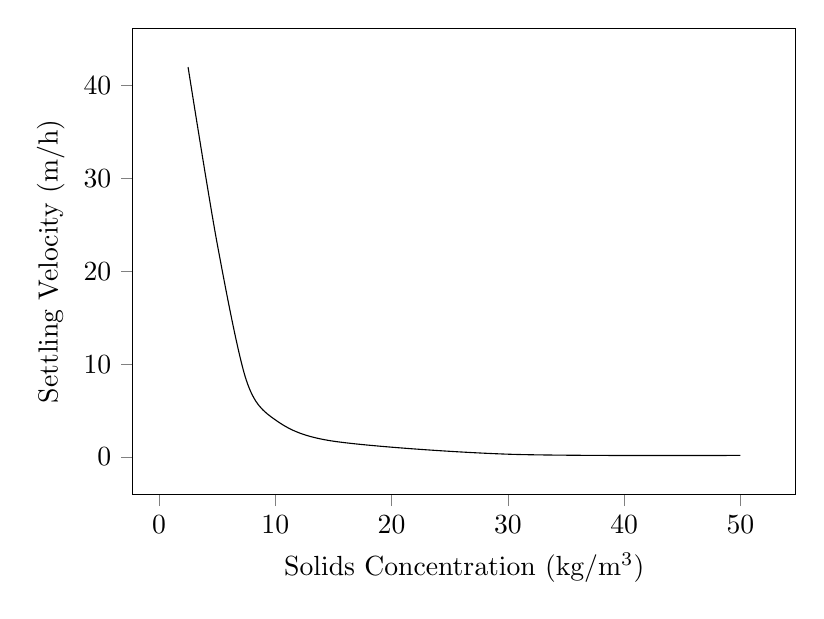
\begin{tikzpicture}
\begin{axis}[
    xlabel={Solids Concentration (kg/m$^3$)},
    ylabel={Settling Velocity (m/h)},
    width=10cm,
    height=7.5cm,
    tick pos=left,
    tick align=outside,
    xtick={0, 10, 20, 30, 40, 50},
    ytick={0, 10, 20, 30, 40, 50},
    smooth
]
\addplot[color=black, mark=none] table {
Solids Concentration Settling Velocity
2.5 42
5 23
7.5 8.3
10 4
15 1.7
30 0.3
50 0.17
};
\end{axis}
\end{tikzpicture}
\captionsetup{font=sl, labelsep=period, labelfont=bf}
\caption{Zone settling velocities (ZSV) in different solid concentrations.}
\label{fig:zsv}
\end{figure}
Since there is no information on the underflow conditions ($Q_u$), \emph{Yoshioka construction} can be used for determining the allowable maximum solids loading ($G_L$) for thickeners to function properly graphically by drawing a tangent line to the solids-flux curve from $C_u$, which intersects ($G_L$) value on Y axis \autocite{sanin2011, Yoshioka1957}.\\
The desired $C_u$ value is 4\% (assuming sludge specific gravity as 1.02):\\
$C_u = 4 \text{ kg}/ 100 \text{ kg}* 1.02 * 1000 \text{ kg/m}^3 = 40.8 \text{ kg/m}^3$

\begin{figure}[htbp]
\centering
\begin{tikzpicture}
\begin{axis}[
    xlabel={Solids Concentration (kg/m$^3$)},
    ylabel={Flux (kg/m$^2$h)},
    tick pos=left,
    width=15cm,
    height=10cm,
    tick align=outside,
    xtick={0, 10, 20, 30, 40, 50},
    ytick={0, 25, 32, 50, 75, 100, 125},
    yticklabels={0, 25, {}, 50, 75, 100, 125},
    smooth,
    extra x ticks={40.8},
    extra x tick labels={}
]
\addplot[color=black, mark=none] table {
Solids Concentration Settling Velocity
2.5 105
5 115
7.5 62.25
10 40
15 25.5
30 9
50 8.5
};
\draw[dashed] (40.8,0) -- (0,32);
\node[anchor=west, font=\footnotesize] at (axis cs:40.8,3) {\fbox{$C_u$ = 40.8 kg/m$^3$}};
\node[font=\footnotesize] at (axis cs:3.5,37) {\fbox{$G_L$ = 32 kg/m$^2$h}};
\end{axis}
\end{tikzpicture}
\captionsetup{font=sl, labelsep=period, labelfont=bf}
\caption{Flux values w.r.t. solid concentrations with Yoshioka construction.}
\label{fig:yoshioka}
\end{figure}

The dashed line originating from $C_u$ value in Figure \ref{fig:yoshioka} yields $G_L$ value as \textbf{32 kg/m\bm{$^2$}h}.\\
For the area calculation:
\begin{equation}
    \text{A} = \frac{C_0Q_0}{G_L} =\frac{\text {Mass loading rate}}{\text {Allowable maximum solids flux}}
    \label{eq:area}
\end{equation}
Since in the question, the initial mass loading rate is already given as 2250 kg/h, using Equation \ref{eq:area}:
$$\text{Area} = \frac{2250 \text{ kg/h} }{32 \text{ kg/m}^2\text{h}} = 70.3125 \text{ m}^2 $$
$$\text{Diameter (m)} = \sqrt{\frac{4*\text{Area}}{\pi}} \approx \boxed{9.5 \text{ m}} $$
\textbf{Comment:} For a circular thickener, around \emph{10 m} diameter is enough for the construction of the thickener functioning efficiently based on experimental data. Although the observed data is crucial while designing the thickener, the hydraulic overflow rate should be suitable for the design as well \autocite{metcalf2014}.
\section{}
According to \textcite{sanin2011, metcalf2014}, two precipitation events occur when Alum is added to wastewater for settlement:\\
\ce{Al^3+ + PO_4^3- \rightleftarrows AlPO4} $\downarrow$ ppt.\\
\ce{Al^3+ + 3OH- \rightleftarrows Al(OH)3} $\downarrow$ ppt.\\
The following calculations are done according to the molecular weights of elements and compounds in Table \ref{tab:mws}.
\begin{table}[htbp]
    \centering
    \captionsetup{font=sl, labelsep=period, labelfont=bf}
    \caption{Molecular weights of elements and compounds for the calculations.}
    \begin{tabular}{cc}
    \toprule
    \textbf{Formula} & \textbf{M.W. (g/mol)} \\
    \cmidrule(lr){1-1} \cmidrule(lr){2-2}
    \ce{Al^3+} & 26.982 \\
    \ce{P^3-} & 30.974 \\
    \ce{O^2-} & 15.999 \\
    \ce{H^+} & 1.008 \\
    \ce{PO4^3-} & 94.971 \\
    \ce{OH^-} & 17.007 \\
    \ce{AlPO4} & 121.953 \\
    \ce{Al(OH)3} & 78.003 \\
    \bottomrule
    \end{tabular}
\label{tab:mws}
\end{table}
\begin{center} \textbf{Sludge Production} \end{center}
\textbf{For the \ce{P} removal part:} 0.8 mg/L residual \ce{P} achieved, which is because there are many versions of \ce{P} in wastewater \autocite{Nobaharan2021}, with the initial concentration of 5.8 mg/L.\\
$5.8\text{ mg/L} - 0.8\text{ mg/L} = 5.0\text{ mg/L \ce{P} removed as sludge.}$\\
$5.0\text{ mg/L} * 121.953\text{ g/mol } / \ 30.974\text{ g/mol} \approx 19.7\text{ mg/L \ce{ AlPO4} precipitated.}$\\
\textbf{Excess Alum addition part:} 21 mg/L \ce{Al(OH)3} is produced.\\
\textbf{Total sludge production:} $19.7\text{ mg/L} + 21 \text{ mg/L} = \boxed{40.7 \text{ mg/L}}$
\begin{center} \textbf{Alum Calculations} \end{center}
\textbf{For the \ce{AlPO4} production part:} $5.0\text{ mg/L} * 26.982\text{ g/mol } / \ 30.974\text{ g/mol} \approx 4.4\text{ mg/L \ce{ Al^3+} is required.}$\\
\textbf{For the \ce{Al(OH)3} production part:} $21\text{ mg/L} * 26.982\text{ g/mol } / \ 78.003\text{ g/mol} \approx 7.3\text{ mg/L \ce{ Al^3+} is required.}$
\textbf{Total Alum requirement:} $4.4\text{ mg/L} + 7.3 \text{ mg/L} = \boxed{11.7 \text{ mg \ce{Al^3+}/L}}$
\vfill
\printbibliography
\end{document}